\documentclass[../uilmath.tex]{subfiles}
\graphicspath{{\subfix{../figures/}}}
\begin{document}
\chapter{Statistics}
\section*{Problems}
\begin{enumerate}[label=\bfseries\arabic*.]
    \item %% Problem 1
    A box contains 5 green balls, 4 blue balls, and 3 red balls. Two balls are randomly selected, one at a time, without replacement. What is the probability that both are blue?

    \item %% Problem 2
    If two dice are rolled at one time, what is the probability that both dice show a prime number?

    \item %% Problem 3
    OVer the last few years, the length of Randy's drives at the local driving range follows a normal distribution with a mean of 
    225 yards and a standard deviation of 6 yards. Approximately what percentage of his drives are between 219 yards and 231 yards? (nearest whole number)

    \item %% Problem 4
    A fair die is rolled four times. What is the probability of getting an even number, a prime number, a Fibonacci number, and a perfect number, in that order?

    \item %% Problem 5
    Mel is throwing darts at a circular target with a diameter of 24. On the raget are two concentric circles with diameters 8 and 16. A dart landing in the small circle earns 10 points.
    A dart landing inside the circle with a diameter of 16, but outside the small circle earns 6 points. A dart landing on the target outside of the two concentric circles earns 2 points.
    Find the expected value of the points earned on any randomly selected toss that lands on the target. (nearest tenth)


    Use the table below for problems 6 and 7. Karen owns the Kwik Stop in Sundown. She believes that the number of water bottles sold each day 
    varies with the temperature. She made a table of the high temperature and the number of water bottles sold on the 15th day of the month, for the months of April through September.
    \begin{center}
        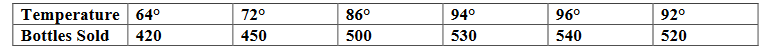
\includegraphics[width=0.8\textwidth]{2021SAC35.PNG}
    \end{center}
    \item %% Problem 6
    Find the sum of the mean, median, and range for the number of water bottles sold on these six days.

    \item %% Problem 7
    Use the data from the table to create an appropriate mathematical model and predict the high temperature on a day that Karen sold 354 water bottles. (nearest whole number)

    \item %% Problem 8
    The preferred swimming pool temperature of adult females follows a normal distribution with a mean of 82$\degree$ F with a standard deviation of $3\degree$ F. Find the probability that a random selected adult female 
    will prefer a temperature between $26\degree$ C and $29\degree$ C. (nearest thousandth)

    \item %% Problem 9
    A researcher took a random sample of 1,000 teenage males in order to estimate the mean number hours of sleep a typical 
    teenage boy gets each night. A 90\% confidence interval would be \blank than a 98\% confidence interval and would involve 
    \blank risk of being incorrect.

    \item %% Problem 10
    A one-stample $t$ statistic from a sample of 40 observations for the two-sided test of 
    \begin{center}
        $H_0 = 26$ \qquad $H_a\neq 26$
    \end{center}
    has the value $t=-1.44$. Find the $p$-value for this test. (nearest thousandth)

    \item %% Problem 11
    When analyzing data, statisticians often report the five-number summary. Which of the following are included in the five-number summary?\\
    I. mean \quad II. standard deviation \quad III. median \quad IV. quartiles \quad V. maximum and minimum

    \item %% Problem 12
    A shipment of twenty refurbished computers contains four defective computers. In how many ways 
    can Rocket purchase five of these computers and get two defective ones?

    \item %% Problem 13
    James has 6 calculus books and 8 physics books on his bookshelf at home. How many arrangements are possible if he keeps the calculus books together and the physics books together?


    \begin{center}
        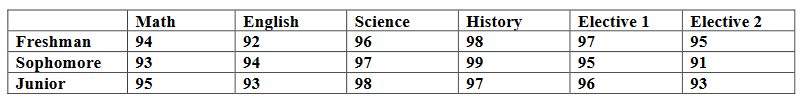
\includegraphics[width=0.8\textwidth]{2022SAC50.PNG}
    \end{center}
    Use the table above for problems 14 and 15.\\
    The table shows the grades for Carolyn her first three years at HPHS.
    \item %% Problem 14
    What is Carolyn's cumulative average after three years of school? (nearest hundredth)

    \item %% Problem 15
    If Carolyn needs to have a cumulative average of 95.45 or higher to graduate in the top 10, what is the minimum 
    average required during her senior year to meet this goal? She plans to take 6 courses her senior year. (nearest hundredth)

    \item %% Problem 16
    Suppose the distribution of the heights of adult males in Nevada is approximately normal with a mean height of 70 inches 
    and a standard deviation of 2.7 inches. A height of 72 inches corresponds to what percentile in the distribution?

    \begin{center}
        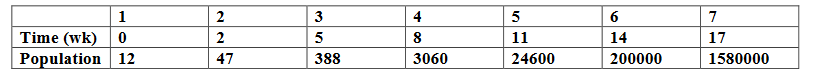
\includegraphics[width=0.8\textwidth]{2022SAC55.PNG}
    \end{center}
    Use the table above for problems 17 and 18.\\
    Sam was doing research for his master's thesis at Harvard. He estimated the population 
    of an isolated group of flies at seven different times. He started at $t=0$ with 12 flies. He finished at $t=17$ weeks with 1,580,000 flies.
    \item %% Problem 17
    Sam entered the data into a list he called $L_1$ and the populations into a list he called $L_2$ on his computer. Which of the following transformation equations will linearize the data?
        
    $\textbf{(A)} (L_1,(L_2)^3) \qquad \textbf{(B)} ((L_1)^3,L_2) \qquad \textbf{(C)} (\log(L_1),L_2) \qquad \textbf{(D)} (L_1,\log(L_2)) \qquad \textbf{(E)} (\log(L_1),\log(L_2))$

    \item %% Problem 18
    Sam was successful in using one of the transformations listed in problem 17 to calculate a regression equation that fit the data. Use this equation 
    to predict how many days after $t=0$ that the population reaches 100,000 flies. (nearest tenth)

    \item %% Problem 19
    Four-hundred students at Texas Tech were randomly selected and asked if they had worked out at the Recreation Center by using a treadmill or an elliptical trainer the past week.
    The results showed that 75 had worked out on both, 190 had worked out on a treadmill, and 260 had worked out on an elliptical trainer. How many of the 400 students 
    stampled had not worked out on either training device the previous week?

    \item %% Problem 20
    Amarillo Slim was playing five card poker. He had a full house, but lost to the dealer who had a royal flush. This is where a player 
    has the ten, jack, queen, king and ace of the same suit. Slim thought the dealer was cheating because the probability of being dealt a royal flush from a standard deck of 52 cards 
    is only $\blank$. (9 decimal places)

    \item %% Problem 21
    Assume that Luka Doncic makes 35.3\% of his 3-point shots regardless of the opponent or where the game is being played. He is 
    unaffected by previous attempts. If he attempts ten 3-points shots in a game, what is the probability that he makes 4, 5, or 6 of the shots? (nearest thousandth)

    \item %% Problem 22
    A survey asked a random sample of 500 U.S. teenagers whether music from the 1970s is superior to music from the 2020s.
    Of the sample, 312 responded with ``yes''. Construct a 95\% confidence interval for the proportion of U.S. teenagers who would say 
    ``yes'' if asked this question.

    \item %% Problem 23
    The average lifetime of battery packs for the Williams Electric vehicle was 4.9 years in 2004. In 2012, they introduced 
    a new battery pack that they believed would last longer. A simple random sample of 50 of the 2012 vehicles with the new battery 
    packs was selected. The mean lifetime of the battery packs turned out to be 5.1 years with a standard deviation of 0.86 years. An appropriate
    test was performed and the resulting $P$-value was $\blank$. (nearest thousandth)

    \item %% Problem 24
    

\end{enumerate}

\section*{Solutions}
\begin{enumerate}[label=\bfseries\arabic*.]
    \item %% Problem 1
    $\frac{1}{11}$

    \item %% Problem 2
    25\%

    \item %% Problem 3
    68\% 

    \item %% Problem 4
    $\frac{1}{36}$

    \item %% Problem 5
    4.2

    \item %% Problem 6
    $1123.\overline{3}$

    \item %% Problem 7
    $46\degree$

    \item %% Problem 8
    0.625

    \item %% Problem 9
    narrower, a greater 

    \item %% Problem 10
    0.158

    \item %% Problem 11
    III, IV, V 

    \item %% Problem 12
    3360

    \item %% Problem 13
    58,060,800

    \item %% Problem 14
    95.17

    \item %% Problem 15
    96.30

    \item %% Problem 16
    77th

    \item %% Problem 17
    D 

    \item %% Problem 18
    91.1 days 

    \item %% Problem 19
    25

    \item %% Problem 20
    .000001539

    \item %% Problem 21
    0.467 

    \item %% Problem 22
    $(.5815, .6665)$

    \item %% Problem 23
    0.053

    \item %% Problem 24
    
\end{enumerate}

\end{document}